
\documentclass[border=10pt]{standalone}
\usepackage{pgfplots}
\pgfplotsset{compat=1.18}
\begin{document}
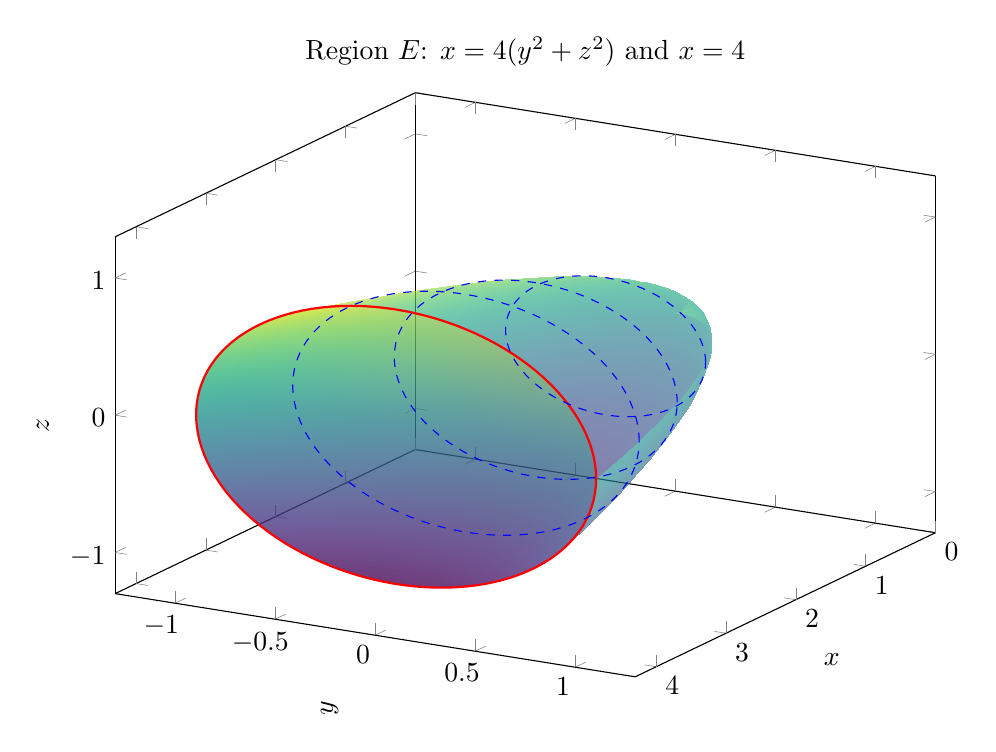
\begin{tikzpicture}
\begin{axis}[
    view={120}{25},
    axis lines=box,
    xlabel=$x$, ylabel=$y$, zlabel=$z$,
    trig format plots=rad,
    domain=0:1, y domain=0:2*pi,
    samples=25, samples y=50,
    colormap/viridis,
    xmin=0, xmax=4.3,
    ymin=-1.3, ymax=1.3, zmin=-1.3, zmax=1.3,
    width=12cm, height=9cm,
    title={Region $E$: $x=4(y^2+z^2)$ and $x=4$},
]
\addplot3[surf, shader=interp, opacity=0.65]
    ({4*x^2}, {x*cos(y)}, {x*sin(y)});
\addplot3[surf, shader=interp, opacity=0.35, fill=orange]
    ({4}, {x*cos(y)}, {x*sin(y)});
\addplot3[domain=0:2*pi, samples=120, samples y=1, thick, red]
    ({4}, {cos(x)}, {sin(x)});
\foreach \xval in {1,2,3} {
    \addplot3[domain=0:2*pi, samples=120, samples y=1, dashed, blue]
        ({\xval}, {sqrt(\xval/4)*cos(x)}, {sqrt(\xval/4)*sin(x)});
}
\end{axis}
\end{tikzpicture}
\end{document}
